% --- CHAPTER 3: METHODOLOGY ---
\chapter{Methodology}
\section{Data Acquisition and Description}

Three primary data sources are used in this project, summarized in Table~\ref{tab:datasets}.

\begin{table}[ht]
\centering
\caption{Summary of datasets used in this project.}
\label{tab:datasets}
\begin{tabular}{@{}lll@{}}
\toprule
\textbf{Dataset} & \textbf{Role} & \textbf{Format} \\
\midrule
ERA5-Land         & Context input      & NetCDF \\
MeteoSwiss TmaxD  & Ground truth       & NetCDF \\
swisstopo DHM25   & Elevation features & Zarr \\
\bottomrule
\end{tabular}
\end{table}

\subsection{ERA5-Land (Context)}

ERA5-Land is the high-resolution land-surface component of the ECMWF ERA5 reanalysis, providing hourly fields on a regular 0.1\textdegree{} latitude--longitude grid from 1950 to the present. Data is downloaded from the Copernicus Climate Data Store as yearly NetCDF files.

\begin{itemize}
    \item \textbf{Variables:} daily maximum 2-meter air temperature (\texttt{t2m\_max}) and the static geopotential field (\texttt{z}).
    \item \textbf{Grid:} 29 latitude $\times$ 61 longitude points over Switzerland (1\,769 cells, $\sim$11\,km spacing).
    \item \textbf{Temporal ranges:} a single year (2023, 365 days) for rapid iteration, and a ten-year window (2014--2023, $\sim$3\,650 days) for the primary experiments.
\end{itemize}

The geopotential field is converted to altitude via $h = z / g$, where $g = 9.80665$\,m/s\textsuperscript{2}. This provides the coarse grid-cell elevation used to compute the elevation difference feature (see Section~\ref{sec:feature_engineering}).

\subsection{MeteoSwiss TmaxD v2.0 (Ground Truth)}

The target observations come from the MeteoSwiss gridded temperature product TmaxD v2.0, derived from station observations using spatial interpolation.

\begin{itemize}
    \item \textbf{Variable:} daily maximum temperature.
    \item \textbf{Grid:} 240$\times$370 points in the Swiss LV95 coordinate system (EPSG:2056), $\sim$1\,km spacing.
    \item \textbf{Units:} degrees Celsius, converted to Kelvin to match the ERA5-Land reference frame before normalization.
    \item \textbf{Coverage:} after flattening, 88\,800 points total, of which a subset are valid (non-NaN) on any given day---points outside the Swiss border are masked.
\end{itemize}

\subsection{swisstopo DHM25 high-Resolution Topography}

Elevation and terrain features are derived from the swisstopo DHM25 (Digital Height Model), stored locally in Zarr format on a 25\,m Swiss LV95 grid (12\,800$\times$14\,200 pixels). The dataset includes pre-computed terrain derivatives.

\begin{itemize}
    \item \textbf{DEM}: surface elevation in meters.
    \item \textbf{TPI\_500M}: Topographic Position Index at a 500\,m radius, quantifying relative elevation compared to the surrounding terrain.
\end{itemize}

These fields are interpolated to target point locations using bilinear interpolation, after converting target coordinates from WGS84 to the LV95 projection.

\section{Data Preprocessing and Exploration}
\label{sec:feature_engineering}

The preprocessing pipeline transforms the three raw datasets into the tensor representations consumed by the ConvCNP. Because the context input (ERA5-Land) and the target observations (MeteoSwiss) live on different grids, in different coordinate systems, and in different units, the main challenges are coordinate alignment, consistent normalization, and the construction of auxiliary features that help the model account for topographic effects. Figure~\ref{fig:grids} illustrates the spatial relationship between the two grids.

\begin{figure}[ht]
    \centering
    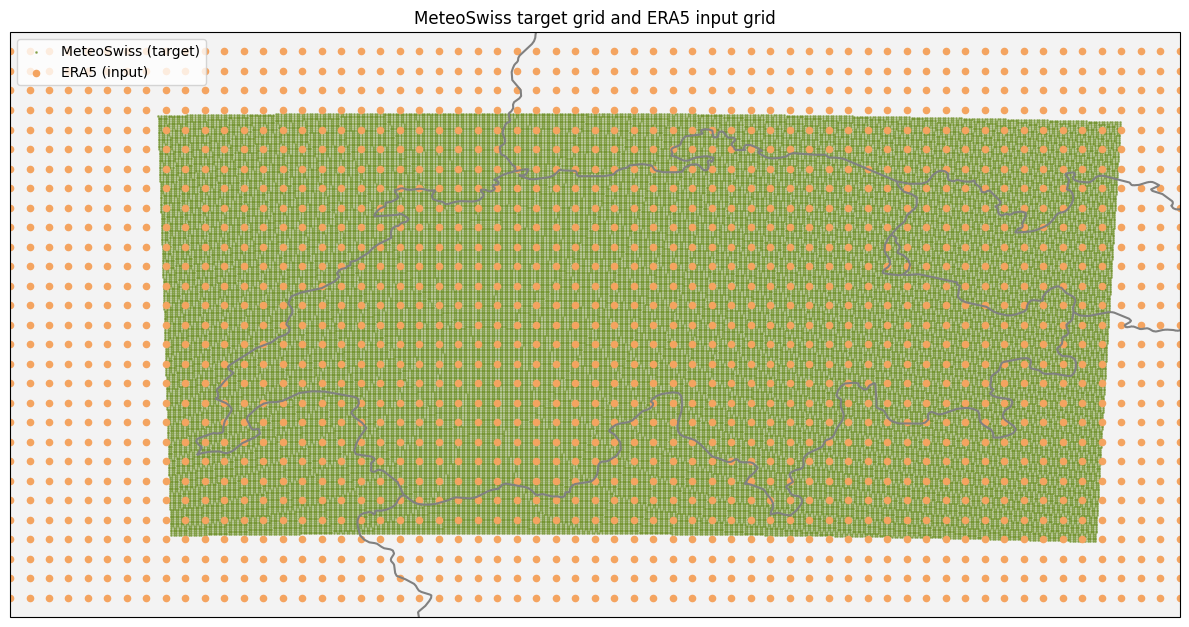
\includegraphics[width=0.85\textwidth]{../dataset_plot.png}
    \caption{Overlay of the ERA5-Land context grid (orange, 29$\times$61 points at $\sim$11\,km spacing) and the MeteoSwiss target grid (green, 240$\times$370 points at $\sim$1\,km spacing). The resolution gap---roughly a factor of 10 in each spatial dimension---is the core downscaling challenge.}
    \label{fig:grids}
\end{figure}

\subsection{Data Quality and Cleaning}

ERA5-Land is a reanalysis product: it is generated by assimilating historical observations into a numerical weather model under rigorous quality control by ECMWF. As a result, the data is spatially and temporally complete---there are no missing values, no gaps in the time series, and no outliers arising from instrument failures. Similarly, the MeteoSwiss TmaxD product is a quality-controlled gridded interpolation of station observations, and the swisstopo DHM25 is a professionally produced digital elevation model. Consequently, no ad-hoc cleaning, gap-filling, or outlier removal was required. The only data filtering applied was temporal subsetting: selecting either a single year (2023, 365 days) for rapid prototyping or a ten-year window (2014--2023, $\sim$3\,650 days) for the primary experiments.

\subsection{Coordinate Alignment and Regridding}

The three datasets use two different coordinate reference systems. ERA5-Land uses a regular latitude--longitude grid in WGS84 (EPSG:4326), while both the MeteoSwiss observations and the swisstopo DEM use the Swiss LV95 projected coordinate system (EPSG:2056), whose axes are expressed in meters. Aligning these required two types of coordinate transformations, both performed using \texttt{pyproj}:

\begin{enumerate}
    \item \textbf{MeteoSwiss $\rightarrow$ ERA5 frame.} The MeteoSwiss dataset provides latitude and longitude fields in WGS84 degrees alongside its native LV95 grid indices. These WGS84 coordinates are normalized to $[0, 1]$ using the ERA5-Land bounding box, so that target locations are expressed in the same reference frame as the context grid.

    \item \textbf{WGS84 $\rightarrow$ LV95 for DEM lookup.} To extract high-resolution elevation at each MeteoSwiss target point, the WGS84 target coordinates are transformed to LV95 meters, then used to query the swisstopo DEM and TPI fields via bilinear interpolation (\texttt{xarray.DataArray.interp}).
\end{enumerate}

The ERA5-Land grid-cell elevation (derived from the geopotential field, see below) is similarly interpolated to target locations, but this interpolation uses the native WGS84 coordinates of the ERA5 grid since both the geopotential and the target latitude/longitude are in the same coordinate system.

\subsection{Feature Engineering}
\label{sec:feature_engineering_details}

\subsubsection{Temperature Normalization}

Both the ERA5-Land context temperatures and the MeteoSwiss target temperatures are normalized using a global Z-score computed from the ERA5-Land training data:
%
\begin{equation}
    \hat{T} = \frac{T - \mu_{\text{ERA5}}}{\sigma_{\text{ERA5}}}
\end{equation}
%
where $\mu_{\text{ERA5}}$ and $\sigma_{\text{ERA5}}$ are the mean and standard deviation of the ERA5-Land \texttt{t2m\_max} field over the entire training period. Using the \textit{same} normalization for both context and target ensures that the model operates in a consistent scale. The MeteoSwiss data, originally in degrees Celsius, is first converted to Kelvin before applying the normalization.

\subsubsection{Coordinate Normalization}

Latitude and longitude are min--max normalized to $[0, 1]$ using the ERA5-Land bounding box:
%
\begin{equation}
    \hat{\phi} = \frac{\phi - \phi_{\min}}{\phi_{\max} - \phi_{\min}}, \qquad
    \hat{\lambda} = \frac{\lambda - \lambda_{\min}}{\lambda_{\max} - \lambda_{\min}}
\end{equation}
%
These normalized coordinates serve two roles: they form two of the five CNN input channels (enabling the model to learn position-dependent patterns), and they define the target locations passed to the decoder.

\subsubsection{Cyclical Seasonal Encoding}

The day of year $d \in \{1, \ldots, 365\}$ is encoded as a pair of cyclical features:
%
\begin{equation}
    c_{\cos} = \cos\!\left(\frac{2\pi(d-1)}{365}\right), \qquad
    c_{\sin} = \sin\!\left(\frac{2\pi(d-1)}{365}\right)
\end{equation}
%
This representation avoids the discontinuity that a raw day-of-year integer would introduce at the year boundary (day 365 $\rightarrow$ day 1). These two channels are broadcast to the full spatial grid and appended to the ERA5-Land input tensor as channels 4 and 5. Additionally, the same seasonal features are optionally fed directly to the elevation MLP, allowing it to learn season-dependent lapse rate corrections (e.g.\ steeper gradients in summer versus temperature inversions in winter valleys).

\subsubsection{Altitude from Geopotential}

The ERA5-Land geopotential field $\Phi$ (in m$^2$\,s$^{-2}$) is converted to grid-cell altitude via:
%
\begin{equation}
    h_{\text{grid}} = \frac{\Phi}{g}, \qquad g = 9.80665 \;\text{m\,s}^{-2}
\end{equation}
%
This provides a coarse ($\sim$11\,km) estimate of the terrain height at each ERA5-Land grid cell. Since the geopotential is static, only the first time step is used. The resulting altitude field is interpolated to target locations via bilinear interpolation and used to compute the elevation difference feature described below.

\subsubsection{High-Resolution Topographic Features}

Three elevation-related features are computed at each MeteoSwiss target point and passed to the elevation MLP:

\begin{enumerate}
    \item \textbf{True elevation} ($h_{\text{true}}$): bilinearly interpolated from the 25\,m swisstopo DEM at the target's LV95 coordinates.

    \item \textbf{Elevation difference} ($\Delta h = h_{\text{true}} - h_{\text{grid}}$): the difference between the true elevation and the ERA5-Land grid-cell elevation interpolated to the same point. This captures the local altitude mismatch that the coarse grid cannot resolve---for instance, a mountain peak that lies within a grid cell whose mean elevation is hundreds of meters lower.

    \item \textbf{Topographic Position Index} (TPI$_{500}$): interpolated from the swisstopo TPI at a 500\,m radius, quantifying whether a target point sits on a ridge (positive TPI), in a valley (negative TPI), or on an open slope (near-zero TPI). This encodes local terrain shape beyond what a single elevation value conveys.
\end{enumerate}

These three features are stacked into a per-point elevation tensor of shape (\textit{n\_points}, 3), which the MLP uses to adjust the CNN's base prediction for local topographic effects.

\subsection{Context Tensor Assembly}

The final ERA5-Land context tensor has shape (\textit{time}, 5, 29, 61), where the five channels are:
%
\begin{enumerate}
    \item Normalized daily maximum temperature $\hat{T}$
    \item Normalized latitude $\hat{\phi}$
    \item Normalized longitude $\hat{\lambda}$
    \item Cosine seasonal encoding $c_{\cos}$
    \item Sine seasonal encoding $c_{\sin}$
\end{enumerate}
%
A pre-computed distance tensor of shape (\textit{n\_target\_points}, 29, 61) stores the squared Euclidean distance from each target location to every ERA5-Land grid cell. This tensor is used by the set convolution encoder to weight context observations according to their proximity to each target.

\subsection{Metadata Preservation for Reproducibility}

All normalization statistics---the global mean and standard deviation of the ERA5-Land temperature field, the latitude and longitude bounding box, and the original coordinate arrays---are encapsulated in an \texttt{Era5Metadata} dataclass and serialized to JSON alongside each trained model. Similarly, the full training configuration (hyperparameters, ablation switches, data paths, and random seeds) is captured in a \texttt{Params} dataclass and persisted in the same manner. This ensures that any trained model can be loaded and used for inference with the exact normalization and configuration parameters that were used during training, without relying on the original data files being accessible. Both dataclasses support round-trip JSON serialization, including special handling for NumPy arrays in the metadata.

\section{Model Selection and Implementation}
\todo{
\begin{itemize}
    \item \textbf{Justification}: Why ConvCNP was chosen over traditional interpolation.
    \item \textbf{Leveraging Vaughan2021}: explain exactly what was changed in their code and why, explain that we are leveraging their model structure, metrics and tooling to build upon
    \item \textbf{Experimental Setup}: Details on training/validation/test splits and cross-validation holdout sets.
    \item \textbf{Tech Stack}: Renku, Python, PyTorch, xarray, and Dask.
\end{itemize}
}